\chapter{Magnetostatica}

\section{Forza di Lorentz}
Una carica in moto in un campo magnetico $\vec{B}$ è soggetta a una forza, detta \textbf{forza di Lorentz} $\vec{F}_B$ tale che:
\begin{displaymath}
	\vec{F}_B = q \vec{v} \times \vec{B}
\end{displaymath}
Poiché $\vec{F}_B$ è perpendicolare a $\vec{v}$, il modulo della velocità non può variare, ma solo la sua direzione.\\
Poiché $\vec{F}_B$ è perpendicolare allo spostamento, non può compiere lavoro sulla particella. Ciò significa che se il campo magnetico è uniforme non varia l'energia della particella.\\\\
Possiamo considerare tre casi:
\begin{itemize}
	\item{$\vec{v}$ parallelo a $\vec{B}$: il prodotto vettoriale è nullo e la particella non è soggetta a forza magnetica.}
    \item{$\vec{v}$ perpendicolare a $\vec{B}$: se $\vec{B}$ è costante, la particella si muove lungo una traiettoria circolare.}
    \item{Caso generale: la particella segue un moto ad elica lungo l'asse $\vec{u}_B$}
\end{itemize}

\subsection{Forza tra due fili paralleli percorsi da corrente}
\begin{figure}[h!]
	\centering
    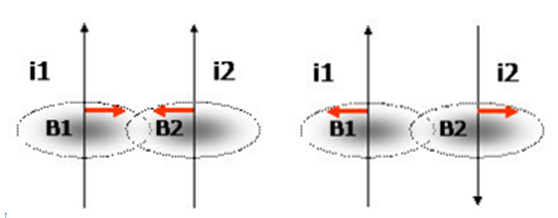
\includegraphics[scale=0.7]{fili-paralleli-corrente.png}
\end{figure}
Un filo rettilineo percorso da corrente $I$ produce, a distanza $r$, un campo magnetico $\vec{B}$:
\begin{displaymath}
	\vec{B} = \mu_0 \cdot \frac{I}{2\pi r}
\end{displaymath}
Consideriamo la seguente configurazione: due fili, di lunghezza $L$, posti a distanza $D$ e percorsi, rispettivamente da una corrente $I_1$ e $I_2$.\\
Sul filo 1 agisce una forza $\vec{F}_{21}$ dovuta a $\vec{B}_2$, mentre sul filo 2 agisce una forza $\vec{F}_{12}$ dovuta a $\vec{B}_1$.\\
\begin{displaymath}\begin{aligned}
	\vec{F}_{21} = L \cdot (\vec{I_1 } \times \vec{B_2}) = I_1 \cdot L \cdot B_2 \cdot \vec{u}_d = 
	I_1 \cdot L \cdot \mu_0 \cdot \frac{I_2}{2\pi \cdot d} \cdot \vec{u}_d\\
	\vec{F}_{12} = L \cdot (\vec{I_2} \times \vec{B_1}) = I_2 \cdot L \cdot B_1 \cdot \vec{u}_d = 
	I_2 \cdot L \cdot \mu_0 \cdot \frac{I_1}{2\pi \cdot d} \cdot \vec{u}_d\\
\end{aligned}\end{displaymath}
Tali forze, secondo la terza legge di Newton sono eguali in modulo e hanno direzioni opposte:
\begin{displaymath}\begin{aligned}
	\vec{F}_{12} = - \vec{F}_{21} =I_1 \cdot L \cdot \mu_0 \cdot \frac{I_2}{2\pi \cdot d} \cdot \vec{u}_d = I_2 \cdot L \cdot \mu_0 \cdot \frac{I_1}{2\pi \cdot d} \cdot \vec{u}_d\\
	F_{12}=F_{21} = \mu_0 \cdot \frac{I_1 \cdot I_2}{2 \pi d}
\end{aligned}\end{displaymath}
La forza è attrattiva se i versi delle correnti sono concordi, mentre è repulsiva se sono discordi.

\section{Legge di Biot-Savart}
La legge di Biot-Savart permette di calcolare il campo magnetico prodotto da un filo percorso da corrente:
\begin{displaymath}
	\vec{B} = \frac{\mu_0}{4\pi} \cdot \int \frac{i \cdot d\vec{s} \times \vec{r}}{r^3}
\end{displaymath}

\subsection{Spira circolare}
Consideriamo una spira circolare di raggio $R$ percorsa da una corrente $I$.\\
Calcoliamo il campo magnetico $\vec{B}$ che essa genera in un punto $P$ posto sull'asse perpendicolare alla spira e passante per il suo centro.\\
$P$ si trova a una distanza $z$ dal centro della spira.
\begin{figure}[h!]
	\centering
	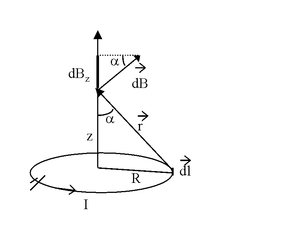
\includegraphics[]{biotSavart.png}
\end{figure}
Scomponiamo $d\vec{B}$ in due componenti:
\begin{itemize}
\item{$dB_z$ lungo l'asse $z$}
\item{$dB_p$ perpendicolare a $dB_z$: per ragioni di simmetria, la somma di tutti i componenti $dB_p$ è nulla}
\end{itemize}
Usiamo la legge di Biot-Savart per calcolare $dBz$:
\begin{displaymath}\begin{aligned}
	dB_z = \mu_0 \cdot \frac{I \cdot \cos{\alpha} \cdot ds}{4\pi \cdot r^2}\\
    r^2 = R^2 + z^2 \qquad \cos{\alpha} = \frac{R}{r} = \frac{R}{\sqrt{R^2 + z^2}}\\
    dB_z = \mu_0 \cdot \frac{I \cdot R}{4\pi \cdot (R^2 + z^2)^\frac{3}{2}}\\
\end{aligned}\end{displaymath}

Il campo magnetico totale $B$ è pari a:
\begin{displaymath}\begin{aligned}
	\vec{B} = \int dB_z \cdot \vec{k} =  \mu_0 \cdot \frac{I \cdot R}{4\pi \cdot (R^2 + z^2)^\frac{3}{2}} \cdot \int dS \cdot \vec{k} = \\
    = \mu_0 \cdot \frac{I \cdot R}{4\pi \cdot (R^2 + z^2)^\frac{3}{2}} \cdot 2 \pi \cdot R \cdot \vec{k} = \\
    =\mu_0 \cdot \frac{I \cdot R^2}{2 \cdot (R^2 + z^2)^\frac{3}{2}} \cdot \vec{k}
\end{aligned}\end{displaymath}

Nel centro della spira ($r=R$):
\begin{displaymath}\begin{aligned}
	\vec{B} = \int dB_z \cdot \vec{k} =  
	\mu_0 \cdot \frac{I \cdot R}{4\pi \cdot (R)^\frac{3}{2}} \cdot \int dS \cdot \vec{k} = \\
    \mu_0 \cdot \frac{I \cdot R}{4\pi \cdot (R)^\frac{3}{2}} \cdot 2 \pi \cdot R  \vec{k} = \mu_0 \cdot \frac{I}{2R} \vec{k}
\end{aligned}\end{displaymath}

\section{Legge di Ampére}
La legge di Ampére ci permette di calcolare la circuitazione del campo magnetico lungo una linea chiusa
\begin{displaymath}
	\oint \vec{B} \cdot d\vec{s} = \mu_0 \cdot I
\end{displaymath}

\subsection{Solenoide ideale}
Un solenoide è caratterizzato da una corrente $I$ che scorre in un filo avvolto a spirale $n$ volte per unità di lunghezza intorno ad un cilindro di raggio $a$ e lunghezza $L$.\\
Se $a <<< L$, il campo magnetico $\vec{B}$ è, in prima approssimazione, contenuto all'interno del solenoide, in direzione assiale, con intensità costante. In queste condizioni (ideali),  
\begin{figure}[h!]
	\centering
	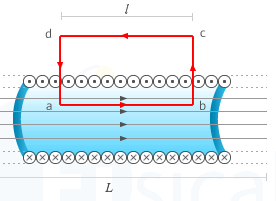
\includegraphics[scale=3]{solenoide-ampere.png}
\end{figure}
\begin{displaymath}\begin{aligned}
	\oint \vec{B} \cdot d\vec{s} = \int_A^B \vec{B} \cdot d\vec{s} + \int_B^C \vec{B} \cdot d\vec{s} + \int_C^D \vec{B} \cdot d\vec{s} + \int_D^A \vec{B} \cdot d\vec{s} + 
\end{aligned}\end{displaymath}
Il secondo e il quarto integrale sono nulli, in quanto o il campo $\vec{B}$ è parallelo al cammino di integrazione (punti interni) o è nullo (punti esterni).\\
Il terzo integrale è nullo perché abbiamo assunto $\vec{B}$ nullo all'esterno del solenoide.
\begin{displaymath}
	\oint \vec{B} \cdot d\vec{s} = \int_A^B \vec{B} \cdot d\vec{s} = B \cdot l\\
\end{displaymath}
Utilizzando la legge di Ampére:
\begin{displaymath}
	B = \mu_0 \cdot \frac{I}{L}
\end{displaymath}

\section{Legge di Faraday-Lenz}
Secondo la legge di Faraday-Lenz, a una variazione del flusso del campo magnetico corrisponde una f.e.m. autoindotta che si oppone a tale variazione.
\begin{displaymath}
	- \frac{d\Phi_S (\vec{B})}{dt} = \epsilon_{indotta}
\end{displaymath}

\subsection{Relazione con induttanza}
Consideriamo un solenoide, in cui $S$ è la superficie della sezione della spira, l'induttanza è $L$ e la corrente che lo percorre è $i(t)$. \
\begin{displaymath}\begin{aligned}
	\Phi_S (\vec{B}) = L \cdot i(t) = \oint \vec{B} \cdot \vec{n}\\
    \frac{d\Phi_S (\vec{B})}{dt} = L \cdot \frac{di}{dt}
\end{aligned}\end{displaymath}
Per la legge di Ampére, al variare del flusso del campo magnetico, il solenoide genera una fem.\\
In particolare, una variazione del flusso avviene al variare della corrente elettrica.
\begin{displaymath}
	\epsilon_{indotta} = -L \cdot \frac{di}{dt}
\end{displaymath}